
\documentclass[]{article}

\title{Ley de números grandes}

\date{}
\usepackage{braket}
\usepackage{bbold}
\usepackage{amsmath,amsfonts,amssymb,amsthm,booktabs}
\usepackage[margin=1.0in]{geometry}
\usepackage{graphicx}
\usepackage{chngcntr}
\usepackage{floatrow}
\usepackage{chngcntr}
\usepackage{hyperref}
\usepackage[spanish]{babel}
\usepackage[svgnames]{xcolor}
\usepackage{commath}
\usepackage{floatrow}
\floatsetup[table]{capposition=top}
\DeclareRobustCommand{\bbone}{\text{\usefont{U}{bbold}{m}{n}1}}

\DeclareMathOperator{\EX}{\mathbb{E}}% expected val
\renewcommand{\spanishtablename}{Cuadro}
\usepackage{listings}
\usepackage[%
    font={small,sf},
    labelfont=bf,
    format=hang,    
    format=plain,
    margin=0pt,
    width=0.8\textwidth,
]{caption}
\usepackage[list=true]{subcaption}
\lstset{language=R,
    basicstyle=\small\ttfamily,
    stringstyle=\color{DarkGreen},
    otherkeywords={0,1,2,3,4,5,6,7,8,9},
    morekeywords={TRUE,FALSE},
    deletekeywords={data,frame,length,as,character},
    keywordstyle=\color{blue},
    commentstyle=\color{DarkGreen},
}

\counterwithin{figure}{section}
\renewcommand*{\figureautorefname}{Figura}


\usepackage[backend=biber]{biblatex}
\addbibresource{ref.bib}

\begin{document}
	\maketitle
	\begin{center}


\centerline{\textbf{TAREA 13} } 
\textbf{ }

\centerline{Alumno: } 
\centerline{Joaquín Arturo Velarde Moreno}


	\end{center}
	

\section{Introducción}

El objetivo de esta tarea es explicar conceptos de probabilidad introducidos en el material del curso \cite{MaterialClase} y ademas con el uso de R poder comprobar numéricamente sus propiedades\cite{rproject},este documento se encuentra alojado en el repositorio\cite{repositorio} como recurso libre .

\section{La desigualdad de Markov}


Es un teorema de la probabilidad, bautizada así por el matemático ruso Andrei Markov, que afirma que la probabilidad que una variable aleatoria $X$ sea como mínimo igual a cierto valor $a$, es a lo mucho la esperanza de esta variable entre el valor $a$, lo cual se puede describir con la formula:
\[ P(\lvert X \lvert \geq a) \leq \frac{\EX(X)}{a}.  \]
Donde:
\begin{itemize}
	\item $X$ es una variable aleatoria.
	\item $a$ es un numero positivo diferente de 0 ($a \in R_{+}^{*}$).
	\item $\EX(X)$ es la esperanza de $X$.
\end{itemize}

Podemos comprobar esta propiedad numéricamente, supongamos que tenemos una distribución de poisson con $n$ datos, un promedio de 3 y asignamos un numero cualquiera para $a$.
  \begin{lstlisting}
a <- 2
n <- 1000
E <- 3
X <- rpois(n,E)
   \end{lstlisting}
Ahora por medio de un \textit{for} obtendremos la probabilidad de que nuestros resultados sean mayor o igual a nuestra $a$.
  \begin{lstlisting}
a <- 2
n <- 1000
E <- 3
X <- rpois(n,E)
contador = 0
for(i in 1:n)
{
  if(abs(X[i]) >= a)
  {
    contador = contador + 1
  }
}
   \end{lstlisting}
Ahora para probar obtendremos la razón de nuestra esperanza entre nuestro numero $a$.
  \begin{lstlisting}
> P <- contador/n
> print(P)
#[1] 0.809
> Cociente <- E/a
> print(Cociente)
#[2] 1.5
   \end{lstlisting}


\section{La desigualdad de Chebyshev}
Es un teorema de la probabilidad formulada por el matemático ruso Pafnuty Chebyshev y maestro de Andrei Markov.
Esta desigualdad es la herramienta básica para demostrar resultados como la ley de los grandes números.
Establece que la probabilidad de que la distancia de una variable aleatoria $X$ a su promedio sea como mínimo un cierto numero $a$, es a lo mucho la varianza entre el cuadrado del numero $a$, el cual se puede describir como:
\[ P(\lvert X - \mu \lvert \geq a) \leq \frac{\sigma^{2}}{a^{2}}.\]
Donde:
\begin{itemize}
	\item $\sigma^{2}$ es la varianza.
	\item $\mu$ es el promedio esperado.
	\item $a$ es un numero positivo diferente de 0 ($a \in R_{+}^{*}$).
\end{itemize}
En resumen establece que la probabilidad de que la distancia de la media sea mayor a cierto numero, es a lo mucho la varianza entre el cuadrado de cierto numero.
Así que si la varianza es pequeña, la probabilidad de estar lejos en la media también es pequeña.
Este teorema puede ser probado por el teorema de Markov, Si analizamos su teorema podremos ver que podemos sustituir elementos de la desigualdad con los de Chebyshev.
\[ P(\lvert X \lvert \geq a) \leq \frac{\EX(X)}{a}.  \]
Donde:
\begin{itemize}
	\item $X = (X - \mu)^{2}$.
	\item $a = \epsilon^{2}$.
\end{itemize}

Si sustituimos nos da algo esencialmente igual al teorema de Chebyshev.
\[ P(\lvert (X-\mu)^{2} \lvert \geq \epsilon^{2}) \leq \frac{\EX(X)}{a}.\]
Nosotros sabemos que $\sigma^{2} = V[X] =\EX[(X-\mu)^{2}]$ y $P(\lvert (X-\mu)^{2} \lvert \geq \epsilon^{2})$ es esencialmente lo mismo que $P(\lvert (X-\mu) \lvert \geq \epsilon)$ por lo tanto nos queda:
\[ P(\lvert X-\mu \lvert \geq \epsilon) \leq \frac{\sigma^{2}}{\epsilon^{2}}.  \]

\section{Ley de números grandes}
Es un teorema fundamental de la probabilidad que indica que si repetimos muchas veces ( que tiende al infinito) un mismo experimento este se acercara a nuestro promedio teórico.
Es decir la probabilidad de que la diferencia entre el promedio analítico y el experimental sea mayor o igual a un numero positivo cuando $n$ se aproxima al infinito es de $0$.
\[ \lim_{n\to\infty} P(\lvert \frac{S_{n}}{n} - \mu \lvert \geq \epsilon) = 0\]
Donde:
\begin{itemize}
	\item $n$ es el números de datos.
	\item $P$ es la probabilidad.
	\item $\epsilon$ es un numero positivo diferente de 0 ($\epsilon \in R_{+}^{*}$).
    \item $\mu$ es el promedio analítico.
	\item $\frac{S_{n}}{n}$ es el promedio experimental.
\end{itemize}
También se establece que la posibilidad de que la diferencia de el promedio analítico y experimental sea menos que un numero positivo cuando n se aproxima al infinito es de 1.
\[ \lim_{n\to\infty} P(\lvert \frac{S_{n}}{n} - \mu \lvert < \epsilon) = 1\]
Donde:
\begin{itemize}
	\item $n$ es el números de datos.
	\item $P$ es la probabilidad.
	\item $\epsilon$ es un numero positivo diferente de 0 ($\epsilon \in R_{+}^{*}$).
    \item $\mu$ es el promedio analítico.
	\item $\frac{S_{n}}{n}$ es el promedio experimental.
\end{itemize}
Este comportamiento se puede comprobar en R\cite{rproject}, imaginemos una distribución normal con \textit{n}  datos, con un promedio de \textit{mu} y una desviación estándar de 2.
  \begin{lstlisting}
n  <- 1000
mu <- 7
de <- 2
x  <- rnorm(n,mu,de)
   \end{lstlisting}
Si por medio de la función \textit{sample} obtenemos el promedio de esos datos tendremos un valor menor o mayor que nuestro promedio analítico.
  \begin{lstlisting}
Sample   <- Sample(x,50)
Promedio <- sum(Sample)/length(Sample)
print(Promedio)
>   print(Promedio)
#[1] 6.574619

   \end{lstlisting}
Si aumentáramos el numero de elementos que tomamos en nuestra muestra eventualmente nuestro promedio experimental y analítico serán cada vez mas cercanos (\autoref{fig:casos}).
\begin{figure}[hbt!]
\centering
\subcaptionbox{Distribución del promedio de una muestra de 5 elementos aleatorios.}{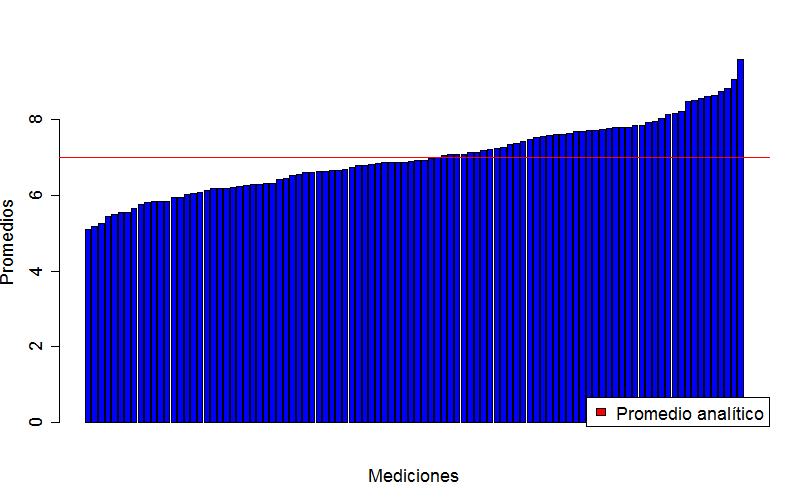
\includegraphics[width=0.5\textwidth]{Figuras/Lng_5.png}}%
\hfill
\subcaptionbox{Distribución del promedio de una muestra de 10 elementos aleatorios.}{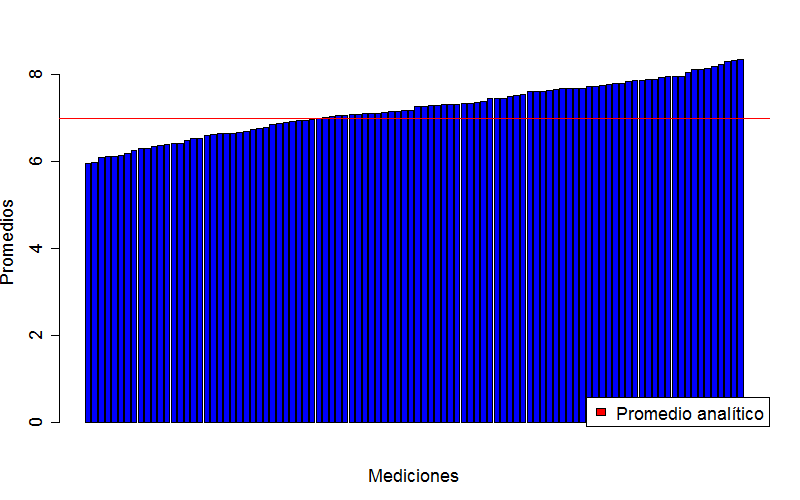
\includegraphics[width=0.5\textwidth]{Figuras/Lng_10.png}}%
\hfill
\subcaptionbox{Distribución del promedio de una muestra de 200 elementos aleatorios.}{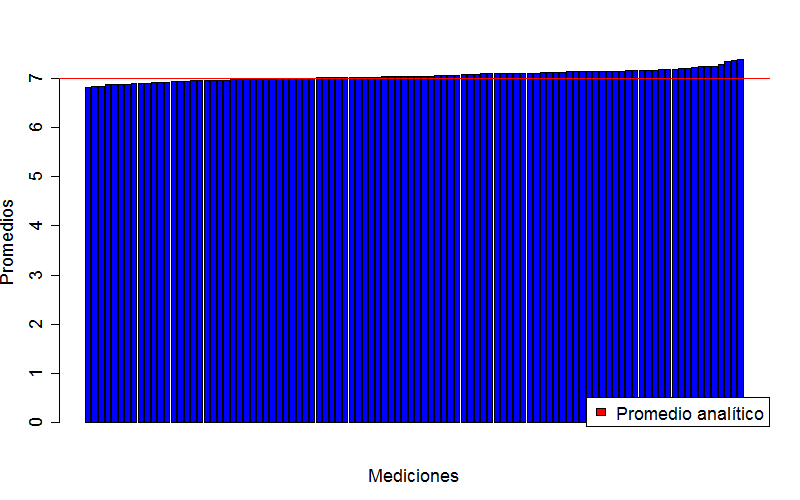
\includegraphics[width=0.5\textwidth]{Figuras/Lng_2000.png}}%
\hfill
\subcaptionbox{Distribución del promedio de una muestra de 1000 elementos aleatorios.}{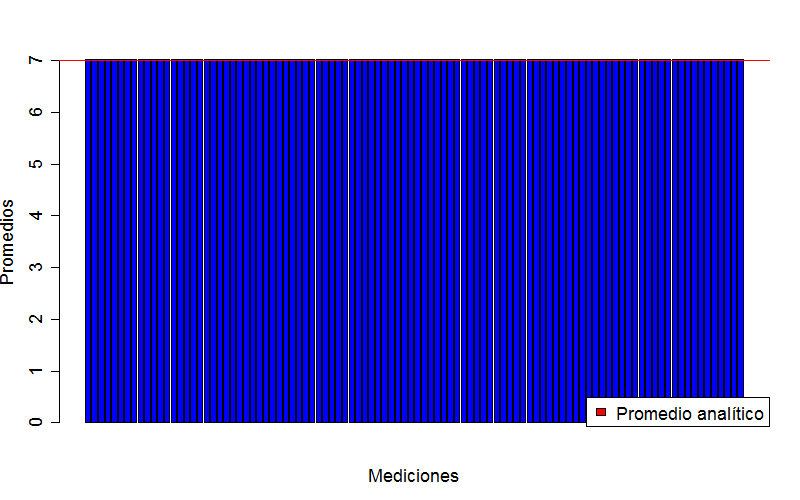
\includegraphics[width=0.5\textwidth]{Figuras/Lng_1000.png}}% 
\hfill
\caption{Distribuciones de promedio en las muestras obtenidas al ir aumentando el número de muestras.}

\label{fig:casos}
\end{figure}   
\hfill
\printbibliography[title={Referencias}]
\end{document}
